\documentclass[14pt,aspectratio=1610]{beamer}

\usepackage[brazil]{babel}
\usepackage[utf8]{inputenc}
%\UseRawInputEncoding
\usepackage[T1]{fontenc}
%\usepackage{Sweave}
\usepackage{animate}
\usepackage{amsbsy}
\usepackage{amsfonts}
\usepackage{amsmath}
\usepackage{amssymb}
\usepackage{amsthm}
\usepackage[toc,page,title,titletoc]{appendix}
%\usepackage[fixlanguage]{babelbib}
%\usepackage[pdftex]{color}
\usepackage{dsfont}
\usepackage{esvect}
\usepackage[labelfont=bf]{caption}
\usepackage{subcaption}
\usepackage{float}
\usepackage[Glenn]{fncychap}%Sonny %Conny %Lenny %Glenn %Renje %Bjarne %Bjornstrup
%\usepackage{geometry, calc, color, setspace}%
%\geometry{a4paper, headsep=1.0cm, footskip=1cm, lmargin=3cm, rmargin=2cm, tmargin=3cm, bmargin=2cm}
\usepackage{graphicx}
\usepackage{indentfirst}%Para indentar os parágrafos automáticamente
\usepackage{lipsum}
\usepackage{longtable}
\usepackage{mathtools}
\usepackage{listings}%Inserir codigo do R no latex
%\usepackage{slashbox}
\usepackage{multirow}
\usepackage{multicol}
\usepackage{natbib}
\setcitestyle{authoryear,open={(},close={)}} %Citation-related commands
\bibliographystyle{abbrvnat}
%\usepackage{csquotes}
%\usepackage[natbib=true,style=abnt, sorting=none]{biblatex}
%\addbibresource{bibliografia.bib}
\usepackage[figuresright]{rotating}
\usepackage{spalign}
%\usepackage{pgfpages}
\usepackage{pgfplots}
\pgfplotsset{compat=1.18}
\usepackage{tikz}
\usepackage{color, colortbl}
\usepackage{ragged2e}%para justificar o texto dentro de algum ambiente
\definecolor{Gray}{gray}{0.9}
\definecolor{LightCyan}{rgb}{0.88,1,1}
\definecolor{Lightblue}{RGB}{50, 149, 168}
%\usepackage{grffile}

\usepackage[all]{xy}



\usetheme{Madrid}
\usecolortheme[RGB={193,0,0}]{structure}

%\setbeamertemplate{footline}[frame number]
%\setbeamertemplate{footline}[text line]{%
%  \parbox{\linewidth}{\vspace*{-8pt}\hfill\date{}\hfill\insertshortauthor\hfill\insertpagenumber}}
\beamertemplatenavigationsymbolsempty
\renewcommand{\vec}[1]{\mbox{\boldmath$#1$}}
\newtheorem{Teorema}{Teorema}
\newtheorem{Proposicao}{Proposição}
\newtheorem{Definicao}{Definição}
\newtheorem{Corolario}{Corolário}
\newtheorem{Demonstracao}{Demonstração}
\newcommand{\bx}{\ensuremath{\bar{x}}}
\newcommand{\Ho}{\ensuremath{H_{0}}}
\newcommand{\Hi}{\ensuremath{H_{1}}}
\everymath{\displaystyle}

\apptocmd{\frame}{}{\justifying}{} % Allow optional arguments after frame.

\title{Estatística I}
\author{Prof. Fernando de Souza Bastos \texorpdfstring{\\ fernando.bastos@ufv.br}{}}
\institute{Departamento de Estatística \texorpdfstring{\\ Universidade Federal de Viçosa}{}\texorpdfstring{\\ Campus UFV - Viçosa}{}}
\date{}
\newcommand\mytext{Aula 13}
\newcommand\mytextt{Fernando de Souza Bastos}
\newcommand\mytexttt{\url{https://ufvest.github.io/}}

\makeatletter
\setbeamertemplate{footline}
{
  \leavevmode%
  \hbox{%
  \begin{beamercolorbox}[wd=.3\paperwidth,ht=2.25ex,dp=1ex,center]{author in head/foot}%
    \usebeamerfont{author in head/foot}\mytext
  \end{beamercolorbox}%
  \begin{beamercolorbox}[wd=.3\paperwidth,ht=2.25ex,dp=1ex,center]{title in head/foot}%
    \usebeamerfont{title in head/foot}\mytextt
  \end{beamercolorbox}%
  \begin{beamercolorbox}[wd=.35\paperwidth,ht=2.25ex,dp=1ex,right]{site in head/foot}%
    \usebeamerfont{site in head/foot}\mytexttt\hspace*{2em}
    \insertframenumber{} / \inserttotalframenumber\hspace*{2ex} 
  \end{beamercolorbox}}%
  \vskip0pt%
}
\makeatother

\providecommand{\arcsin}{} \renewcommand{\arcsin}{\hspace{2pt}\textrm{arcsen}}
\providecommand{\sin}{} \renewcommand{\sin}{\hspace{2pt}\textrm{sen}}
%\newtheorem{Teorema}{Teorema}
%\newtheorem{Proposicao}{Proposição}
%\newtheorem{Definicao}{Definição}
%\newtheorem{Corolario}{Corolário}
%\newtheorem{Demonstracao}{Demonstração}

\titlegraphic{\hspace*{8cm}\href{https://fsbmat-ufv.github.io/}{
\includegraphics[width=2cm]{figs/mylogo.png}}
}


\usepackage{hyperref,bookmark}
\hypersetup{
  colorlinks=true,
  linkcolor=blue,
  citecolor=red,
  filecolor=blue,
  urlcolor=blue,
}

% Layout da pagina
\hypersetup{pdfpagelayout=SinglePage}
\begin{document}
%\Sconcordance{concordance:Aula21.tex:Aula21.Rnw:%
1 251 1 1 8 1 2 6 0 1 1 9 0 1 3 7 1 1 8 7 0 2 1 5 0 2 1 9 0 1 3 76 1 1 %
2 1 0 5 1 5 0 2 1 5 0 1 1 6 0 1 2 7 1 1 2 1 0 4 1 8 0 1 2 4 0 1 2 6 1 1 %
2 1 0 1 1 9 0 1 2 17 1 1 5 4 0 1 1 8 0 1 2 7 1 1 2 1 0 1 1 8 0 1 1 7 0 %
1 1 7 0 2 1 5 0 2 1 9 0 1 2 9 1}


\frame{\titlepage}

\begin{frame}{}
\frametitle{\bf Sumário}
\tableofcontents
\end{frame}

\section{Modelos Probabilísticos}
\begin{frame}{Modelos Probabilísticos}
\frametitle{}
\begin{block}{}
\justifying
Algumas variáveis aleatórias adaptam-se muito bem a uma série de problemas
práticos. Portanto, um estudo pormenorizado dessas variáveis é de grande importância
para a construção de modelos probabilísticos para si\-tua\-ções reais e a consequente
estimação de seus parâmetros. Para algumas dessas distribuições existem tabelas que
facilitam o cálculo de probabilidades, em função de seus parâmetros. Nesta seção
iremos estudar alguns desses modelos, procurando enfatizar as condições em que eles
aparecem, suas funções de probabilidade, parâmetros e como calcular probabilidades.
\end{block}
\end{frame}

\section{Distribuição Uniforme Discreta}
\begin{frame}{Distribuição Uniforme Discreta}
\frametitle{}
\begin{block}{}
\justifying
Este é o caso mais simples de v.a. discreta, em que cada valor possível ocorre com
a mesma probabilidade.\\
{\bf Definição:} A v.a. discreta $X,$ assumindo os valores $x_{1},\cdots, x_{k},$ tem distribuição uniforme se, e somente se,
$$P(X=x_{i})=p(x_{i})=\dfrac{1}{k},\quad \forall\quad i=1,2,\cdots,k.$$
\end{block}
\end{frame}

\begin{frame}{}
\frametitle{}
\begin{block}{}
\justifying
É fácil verificar que,

$$
E(X)=\dfrac{1}{k}{\displaystyle \sum_{i=1}^{k}x_{i}},\quad 
Var(x)=\dfrac{1}{k}\Biggl\{{\displaystyle \sum_{i=1}^{k}x_{i}^{2}}-\dfrac{{\displaystyle\left(\sum_{i=1}^{k}x_{i}\right)^{2}}}{k} \Biggl\}
$$

\end{block}
\end{frame}

\begin{frame}{}
\frametitle{}
\begin{block}{}
\justifying
\begin{figure}[H]
    \centering
    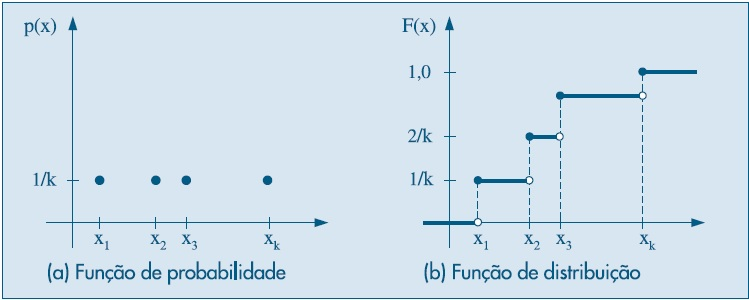
\includegraphics[scale=0.5]{figs/Uniforme}
    \caption{Distribuição uniforme discreta.} %(\cite{Morettin09})}
    %\label{figRotulo}
  \end{figure}

\end{block}
\end{frame}

\begin{frame}{}
\frametitle{Exemplo}
\begin{block}{}
\justifying
Seja $X$ a v.a. que indica o ``número de pontos marcados na face superior
de um dado", quando ele é lançado. Obtemos na Tabela abaixo a distribuição de X.
\begin{table}[h]
\begin{tabular}{c|c|c|c|c|c|c|c}
\hline
x&1&2&3&4&5&6&Total\\
\hline
$p(x)$&$\frac{1}{6}$&$\frac{1}{6}$&$\frac{1}{6}$&$\frac{1}{6}$&$\frac{1}{6}$&$\frac{1}{6}$&1\\
\hline
\end{tabular}
\end{table}
Notemos que $$E(X)=3,5\quad \textrm{e}\quad V(X)=2,9$$
\end{block}
\end{frame}

\section{Distribuição Bernoulli}
\begin{frame}{Distribuição Bernoulli}
\frametitle{}
\begin{block}{}
\justifying
Muitos experimentos são tais que os resultados apresentam ou não uma determinada
característica. Por exemplo:
\begin{enumerate}
\item uma moeda é lançada: o resultado ou é cara, ou não (ocorrendo, então, coroa); \pause
\item um dado é lançado: ou ocorre face 5 ou não (ocorrendo, então, uma das faces
1, 2, 3, 4 ou 6);\pause
\item uma peça é escolhida ao acaso de um lote contendo 500 peças: essa peça é
defeituosa ou não;\pause
\item uma pessoa escolhida ao acaso dentre 1.000 é ou não do sexo masculino;\pause
\item uma pessoa é escolhida ao acaso entre os moradores de uma cidade e verifica-se
se ela é favorável ou não a um projeto municipal.
\end{enumerate}
\end{block}
\end{frame}

\begin{frame}{}
\frametitle{}
\begin{block}{}
\justifying
Em todos esses casos, estamos interessados na ocorrência de sucesso (cara, face 5
etc.) ou fracasso (coroa, face diferente de 5 etc.). Essa terminologia (sucesso e fracasso) será usada freqüentemente.
\end{block}
\pause
\begin{block}{}
\justifying
Para cada experimento acima, podemos definir uma v.a. $X,$ que assume apenas
dois valores: $1,$ se ocorrer sucesso, e $0,$ se ocorrer fracasso. Indicaremos por $p$ a probabilidade de sucesso, isto é, $P(sucesso) = P(S) = p, 0 < p < 1.$
\end{block}
\end{frame}

\begin{frame}{}
\frametitle{}
\begin{block}{}
\justifying
{\bf Definição:} A variável aleatória $X,$ que assume apenas os valores $0$ e $1,$ com função de probabilidade $(x, p(x))$ tal que
\begin{align*}
p(0) &= P(X = 0) = 1 - p,\\
p(1) &= P(X = 1) = p,
\end{align*}
é chamada variável aleatória de Bernoulli.
\end{block}
\pause
\begin{block}{}
\justifying
{\bf Observação:} Experimentos que resultam numa v.a. de Bernoulli são chamados ensaios de Bernoulli. Usaremos a notação $$X\sim Ber(p)$$
para indicar uma v.a. com distribuição de Bernoulli com parâmetro $p.$
\end{block}
\end{frame}

\begin{frame}{}
\frametitle{}
\begin{block}{}
\justifying
Segue-se facilmente que
$$E(X)=p\quad Var(X)=p-p^{2}=p(1-p)$$
e,
$$
F(x)=\left\{
\begin{array}{ccccc}
0,           & \textrm{se} & x<0     ;\\
1-p,& \textrm{se} & 0\leq x<1;\\
1,           & \textrm{se} & x\geq 1 .\\
\end{array}
\right.
$$

\end{block}
\end{frame}

\begin{frame}{}
\frametitle{}
\begin{block}{}
\justifying
\begin{figure}[H]
    \centering
    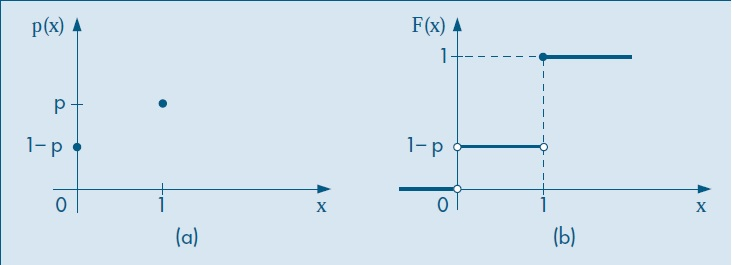
\includegraphics[scale=0.5]{figs/Bernoulli}
    \caption{Distribuição de Bernoulli (a) f.p. (b) f.d.a.} %(\cite{Morettin09})}
    %\label{figRotulo}
  \end{figure}

\end{block}
\end{frame}

\section{Distribuição Binomial}
\begin{frame}{}
\frametitle{Distribuição Binomial}
\begin{block}{}
\justifying
Imagine, agora, que repetimos um ensaio de Bernoulli $n$ vezes, ou, de maneira
alternativa, obtemos uma amostra de tamanho $n$ de uma distribuição de Bernoulli.
Suponha ainda que as repetições sejam independentes, isto é, o resultado de um ensaio
não tem influência nenhuma no resultado de qualquer outro ensaio. Uma amostra
particular será constituída de uma seqüência de sucessos e fracassos, ou, alternativamente, de uns e zeros.
\end{block}
\end{frame}

\begin{frame}{}
\frametitle{Distribuição Binomial}
\begin{block}{}
\justifying
Por exemplo, repetindo um ensaio de Bernoulli cinco vezes $(n = 5),$ um particular resultado pode ser FSSFS ou a quíntupla ordenada $(0, 1, 1, 0, 1).$ Usando a notação 
$P(S) = p,$ a probabilidade de tal amostra será:
$$(1-p)pp(1-p)p=p^{3}*(1-p^{2})$$
O número de sucessos nessa amostra é igual a 3, sendo 2 o número de fracassos.
\end{block}
\end{frame}

\begin{frame}{}
\frametitle{Distribuição Binomial}
\begin{block}{}
\justifying
Designamos por $X$ o número total de sucessos em $n$ ensaios de Bernoulli, com
probabilidade de sucesso $p, 0 < p < 1.$ Os possíveis valores de $X$ são $0, 1, 2, ..., n$ e os pares $(x, p(x)),$ onde $p(x) = P(X = x),$ constituem a chamada distribuição binomial.
\end{block}
\end{frame}

\begin{frame}{}
\frametitle{Distribuição Binomial}
\begin{block}{}
\justifying
Assim, numa seqüência de n ensaios de Bernoulli, a probabilidade de obter $x$ sucessos (e portanto $n-x$ fracassos), $x = 0,1,2, ..., n,$ com $P(S) = p, P(F) = 1-p = q,$ é dado por $p^{x}(1-p)^{n-x}=p^{x}q^{n-x},$ devido à independência dos ensaios. Mas qualquer seqüência com $x$ sucessos e $n-x$ fracassos terá a mesma probabilidade. Portanto resta saber quantas seqüências com a propriedade especificada podemos formar. É fácil ver que existem $$\binom{n}{x}=\dfrac{n!}{x!(n-x)!},$$ logo, 
$$P(X=x)=\binom{n}{x}p^{x}q^{n-x},\ x = 0,1,2, ..., n.$$
\end{block}
\end{frame}

\begin{frame}{}
\frametitle{Distribuição Binomial}
\begin{block}{}
\justifying
Se X tem distribuição binomial com parâmetros $n$ e $p,$ indicamos $X\sim Bin(n,p).$ Nesse caso, 
\begin{align*}
E(X)&=np;\\
V(X)&=np(1-p)
\end{align*}
\end{block}
\end{frame}

\section{Distribuição de Poisson}
\begin{frame}{Distribuição de Poisson}
\frametitle{}
\begin{block}{}
\justifying
Dizemos que uma v.a. $N$ tem uma distribuição de Poisson com parâmetro
$\lambda > 0$ se,

$$P(N=k)=\dfrac{\exp{(-\lambda)}\lambda^{k}}{k!},\ k=0,1,2,\cdots,$$

Neste caso, $E(N)=Var(N)=\lambda;$ Logo, $\lambda$ representa o número médio de eventos ocorrendo no intervalo considerado.

\end{block}
\end{frame}

\begin{frame}{}
\frametitle{}
\begin{block}{}
\justifying
A distribuição de Poisson é largamente empregada quando se deseja contar o número
de eventos de certo tipo que ocorrem num intervalo de tempo, ou superfície ou 
volume. São exemplos:
\begin{itemize}
\item número de chamadas recebidas por um telefone durante cinco minutos;
\item número de falhas de um computador num dia de operação; e
\item número de relatórios de acidentes enviados a uma companhia de seguros numa
semana.
\end{itemize}
\end{block}
\end{frame}

\begin{frame}{Exemplo}
\frametitle{}
\begin{block}{}
\justifying
Um telefone recebe, em média, cinco chamadas por minuto. Supondo que a distribuição de Poisson seja adequada nessa situação, obter a probabilidade de que o telefone não receba chamadas durante um intervalo de um minuto.
\pause
{\bf Resolução:}

$N=$``Número de chamadas por minuto"

Notemos que $\lambda=E(N)=5,$ portanto:

$$P(N=0)=\dfrac{5^{0}\exp{(-5)}}{0!}=0,0067.$$

\end{block}
\end{frame}


\begin{frame}{}
\frametitle{}
\begin{block}{}
\justifying
Por outro lado, se quisermos a probabilidade de obter no máximo duas chamadas
em quatro minutos, teremos $\lambda=20$ chamadas em quatro minutos, logo
\begin{align*}
P(N\leq 2)&=P(N=0)+P(N=1)+P(N=2)\\
&=\exp{(-20)}(1+20+200)\\
&=221\exp{(-20)}
\end{align*}

\end{block}
\end{frame}

\begin{frame}{}
\frametitle{}
\begin{block}{}
\justifying
Denotaremos uma v.a. $N$ com distribuição de Poisson de parâmetro $\lambda$ por:

$$N\sim Poisson(\lambda)$$
\end{block}
\nocite{Apostila}
\end{frame}

\begin{frame}%[allowframebreaks]
\frametitle{\bf Referências}
\bibliography{Referencias/Referencias.bib}
\end{frame}


\end{document}
